\section{Introduction}

This labwork goal is to design, optimize and simulate a Recycling Folded-Cascode (RFC) operational transconductance amplifier (OTA) circuit\textsuperscript{\cite{artigo-prof}}.
The circuit was designed using the TSMC 65nm technology and the simulation using the Cadence Virtuoso software. In Figure \ref{fig:OTA_schematic} is the proposed circuit schematic.

\begin{figure}[H]
    \centering
    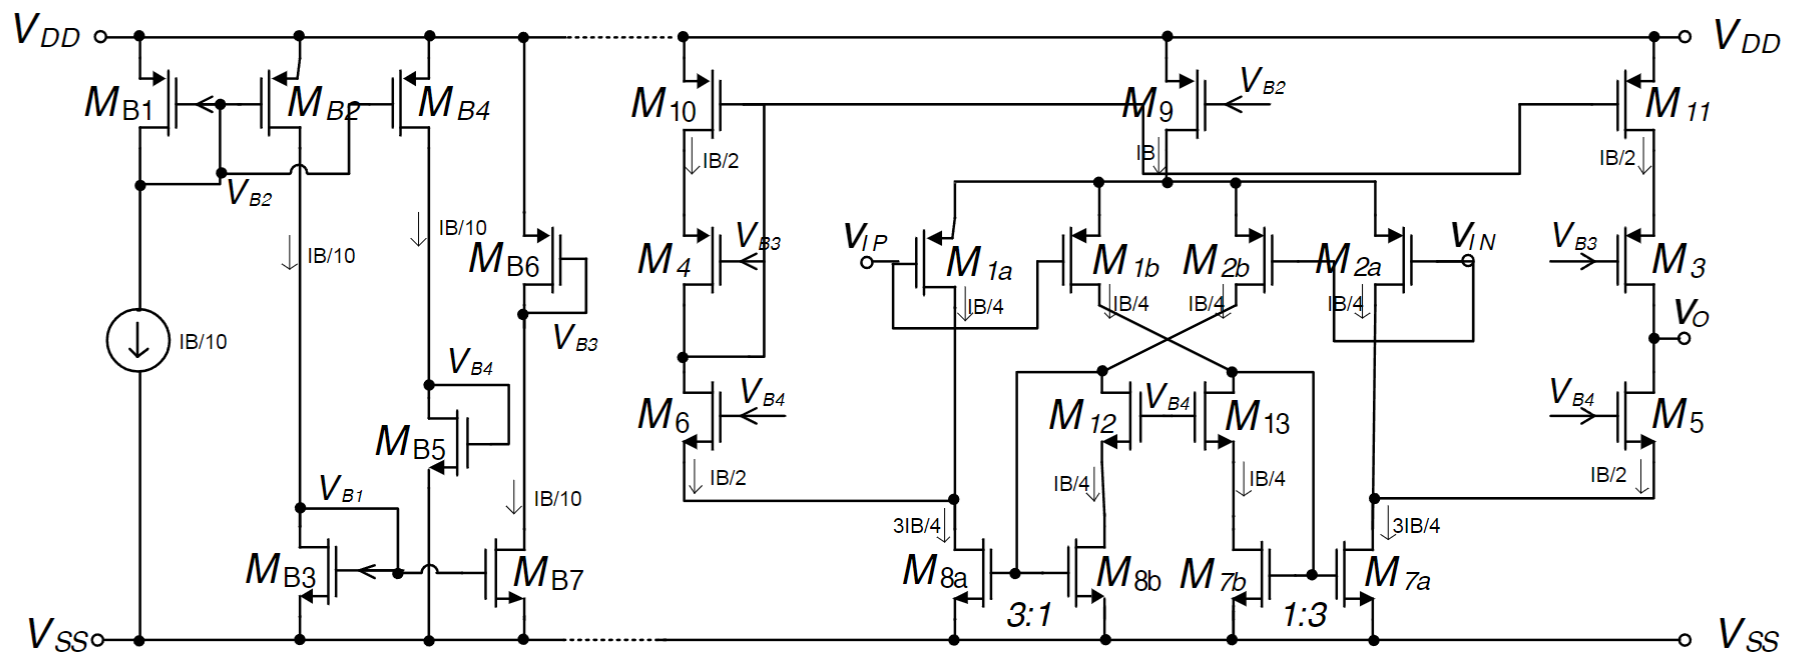
\includegraphics[width=1\textwidth]{Images/RFC_OTA_schematic.png}
    \caption{Recycling Folded Cascode OTA Schematic\textsuperscript{\cite{Lab-statement}}}
    \label{fig:OTA_schematic}
\end{figure}

\begin{table}[H]
    \centering
    \caption{Goals and Constraints}
    \begin{tabularx}{\textwidth}{>{\centering\arraybackslash}X >{\centering\arraybackslash}X}
        \toprule
        \textbf{Goal/Constraint} & \textbf{Description}\\
        \midrule
        DC Gain & $A_{min}\geq \SI{66}{\decibel}$\\
        \midrule
        Gain Bandwidth Product ($C_L = \SI{2}{\pico\farad}$) & $GBW\geq\SI{100}{\mega\hertz}$ \\
        \midrule
        Second Pole Frequency & $f_{p2}>>\SI{200}{\mega\hertz}$ \\
        \midrule
        Third Pole Frequency & $f_{p3} \geq \SI{1}{\giga\hertz}$ \\
        \midrule
        Output Swing ($V_{margin}=\SI{80}{\milli\volt}$) & $OS\geq 0.5 V_{p.p}$ \\
        \midrule
        Channel Lengths & $\SI{180}{\nano\meter} \leq L's \leq \SI{1}{\micro\meter} $ \\
        \midrule
        Moderate Inversion & $\SI{50}{\milli\volt} \leq V_{DSat} \leq \SI{150}{\milli\volt}$ \\
        \midrule
        Excess-Noise Factor & $\Gamma \leq 3.5 $\\
        \bottomrule
    \end{tabularx}
    \label{tab:goals}
\end{table}

The design was simulated, and the results were analyzed and compared to the theoretical values. The results were then used to calculate the merit of the circuit. The results were compared with those in Table \ref{tab:goals}, to ensure the specifications were met.

\pagebreak

